\documentclass[../main.tex]{subfiles}
\graphicspath{{\subfix{../IMAGES/}}}

\begin{document}
\localtableofcontents
Model for optimization : \begin{itemize}
    \item Decision variables : $x \in \mathbb{R}^n$\\
    \item Objective function : $f(x) \in \mathbb{R}$\\
    \item Constraints : $x \in X \subseteq \mathbb{R}^n$\\
\end{itemize}

\quad \underline{Equivalence :} Problems P1 and P2 are equivalent if a feasible point of P1 can be created from a feasible point of P2, with the same value of the objective function.\\

We have the relation : \begin{equation}
    \begin{split}
        \min f(x) = - \max -f(x)\\
        \text{argmin} f(x) = \text{argmax} -f(x)\\
    \end{split}
\end{equation}

\quad \underline{Equality and inequality constraints :} \begin{equation}
    g(x) = 0 \Leftrightarrow \begin{cases}
        g(x) \leq 0 \\
        g(x) \geq 0\\
    \end{cases}
\end{equation}

\quad \underline{Non negative variables :} \begin{equation}
    x \in \mathbb{R}, x = x^+ - x^-
\end{equation}

\quad \underline{Translation :} Constraint $x \geq a$. Change of variable : $x = \Tilde{x}+a$ constraint becomes $\Tilde{x}\geq 0$.\\

\quad \underline{Slack variables :} We have two types \begin{itemize}
    \item Linear : \begin{equation}
        g(x) \leq 0 \Leftrightarrow \begin{cases}
            g(x) + y =0\\
            y \geq 0\\
        \end{cases}
    \end{equation}
    \item Non linear : \begin{equation}
        g(x)\leq 0 \Leftrightarrow g(x) +z^2 =0\\
    \end{equation}
\end{itemize}

\quad \underline{Problem definition :}\\
Objective function : $\min_{x\in \mathbb{R}^n} f(x)$ $f:\mathbb{R}^n\rightarrow \mathbb{R}, n>0$\\
subject to : \begin{itemize}
    \item equality constraint $h(x)=0$, $h: \mathbb{R}^n \rightarrow \mathbb{R}^m$, m>0 the number of constraint\\
    \item inequality constraint $g(x) \leq 0$, $g: \mathbb{R}^n \rightarrow \mathbb{R}^p$, p>0 the number of constraint
\end{itemize}

\quad \underline{Feasible set :} the set of solution of x that satisfies the problem. \\
\begin{equation}
    Y = \{ x\in \mathbb{R}^n | h(x)=0, g(x)\leq 0 \text{ and } x\in X\}
\end{equation}

Which leads to :\\
$\min_{x\in \mathbb{R}^n}$\\
subject to : $x\in Y$\\

\subsection{Linear optimization}

The problem in standard form can be written either as : \\
\begin{minipage}{.5\textwidth}
    \begin{equation}
        \min_{x\in \mathbb{R}^n} \sum_{i=1}^n c_ix_i
    \end{equation}
    subject to \begin{equation}
        \begin{split}
            \sum_{i=1}^n a_{ij}x_i = b_j & j=1,\dots, m\\
            x_i \geq 0 & i=1,\dots, n
        \end{split}
    \end{equation}
\end{minipage}
\vline
\begin{minipage}{.5\textwidth}
    \begin{equation}
        \min_{x\in \mathbb{R}^n} c^T x
    \end{equation}
    subject to \begin{equation}
        \begin{split}
            Ax=b\\
            x\geq 0
        \end{split}
    \end{equation}
    Where $A \in \mathbb{R}^{mxn}$, $b\in \mathbb{R}^m$ and $c\in \mathbb{R}^n$
\end{minipage}

It is convenient to write linear constraints in standard form. All inequality constraints are \textbf{non-negative constraints}. The rest are equality constraints.\\

\subsubsection{Polyhedron}
We can also write the solution set as (canonical form, here A includes the constraints on x such as $x>0$) : \begin{equation}
    \mathcal{P} = \{x \in \mathbb{R}^n | Ax\leq b\}
\end{equation}

Or in standard form : \begin{equation}
    \mathcal{P} = \{x \in \mathbb{R}^n |Ax = b, x\geq 0\}
\end{equation}

\warning A polyhedron is a convex set : \begin{theoremen}
    For all x,y $\in \mathcal{P}$, for all $0\leq \lambda \leq 1$, \begin{equation}
        \lambda x + (1-\lambda)y \in \mathcal{P}
    \end{equation}
\end{theoremen}

\subsubsection{Active constraints}
An active constraint is one that matters. In linear optimization, finding the optimum solution amounts to finding the constraints that are active at the solution.\\

\begin{minipage}{.5\textwidth}
    \underline{Inequality constraints :}\\
    Consider $g:\mathbb{R}^n \rightarrow \mathbb{R}$ and the constraint $g(x)\leq 0$\\
    It is active at $x^*$ if : $g(x^*)=0$\\
\end{minipage}
\vline
 \begin{minipage}{.5\textwidth}
    \underline{Equality constraints :}\\
    Consider $g:\mathbb{R}^n \rightarrow \mathbb{R}$ and the constraint $g(x)= 0$\\
    It is active at $x^*$ if : $g(x^*)=0$\\
\end{minipage}

\subsubsection{Redundant constraints}
\begin{theoremen}
    Consider a compatible system $Ax=b$, $A \in \mathbb{R}^{mxn}$, $b\in \mathbb{R}^m$.\\
\begin{equation}
    \text{Rank}(A) = r<m
\end{equation}
There exists \textbf{m-r redundant constraints that can be removed}.\\
\end{theoremen}

\subsubsection{Feasible direction}
Consider $Y \subseteq \mathbb{R}^n$, the feasible set and $x\in Y$\\
The direction $d\in \mathbb{R}^n$ is feasible in $x$ if $\exists \eta>0$ such that \begin{equation}
    x+\alpha d \in Y, \forall 0<\alpha<\eta
\end{equation}

A feasible direction is a direction that you can take from a specific point and stay in the solution set.\\

There are two conditions for d to be feasible in a convex set : \begin{itemize}
    \item $Ad = 0$\\
    \item if $x_i^+ >0, \forall i$ : every direction if feasible. Otherwise, if $\exists i$ such that $x_i^+ = 0$ then $d_i>0$
\end{itemize}
They both come from the fact that : $x^+\in \mathcal{P}$, $d\in \mathbb{R}^n$, $\alpha >0$ we have $b = Q(x^+ + \alpha d) = Ax^+ + \alpha A d = b + \alpha A d \Rightarrow b$\\

\subsubsection{Elimination of constraints}
If the polyhedron is in standard form, we use the equality constraints to eliminate some of them (the basic variables).\\

\quad \underline{Method :}\\
\begin{equation}
    Ax=b, A\in \mathbb{R}^{mxn}, b\in \mathbb{R}^m, x\in \mathbb{R}^n, \text{rank}(A)=m
\end{equation}
We have $P$ a transformation matrix. We want to separate A into two matrix B (matrix containing the basic vectors) and N (the non-basic ones). B has to be squared : $B \in \mathbb{R}^{mxm}$ and its column have to be linearly independent.\\
We can also compute : $n-m$ non basic variables.\\
We also have the relation $PP^T = I$\\
\begin{equation}
    AP = (B|N)
\end{equation}

We can therefore write : $Ax = Bx_B + Nx_n = b$\\
By doing so, we can finally eliminate the basic variables and get their values with : \begin{equation}
    x_B = B^{-1} (b-Nx_n)
\end{equation}

\subsubsection{Vertices}
The vertices of a polyhedron play a major role in optimization as this is where we will often find the optimal solution.\\

$x$ is a vertex of $\mathcal{P}$ if there is no $y,z\in \mathcal{P}$ such that $\exists 0<\lambda<1$ and $x=\lambda y+ (1-\lambda)z$\\

At a vertex, constraints are active, therefore we have $x_i=0$. \\
To find a vertex : \begin{itemize}
    \item Select and eliminate basic variables\\
    \item Set all non basic variables to 0\\
    \item Check feasibility : $x_B = B^{-1}b \geq 0$\\
\end{itemize}

\begin{equation}
    x = P\begin{pmatrix}
        B^{-1}(b-Nx_n)\\
        x_n\\
    \end{pmatrix} = P \begin{pmatrix}
        B^{-1}b\\
        0_{\mathbb{R}^{n-m}}\\
    \end{pmatrix}
\end{equation}

\begin{theoremen}
    $x^* \in \mathcal{P}$ is a vertex of $\mathcal{P}$ if and only if it is a feasible basic solution.\\
\end{theoremen}

\subsubsection{Degeneracy}
\begin{equation}
    \mathcal{P} = \{x \in \mathbb{R}^n | Ax=b, x \geq 0\}, A \in \mathbb{R}^{mxn}, b\in \mathbb{R}^m
\end{equation}
A basic solution $x$ is degenerate if \begin{itemize}
    \item more than n constraints are active at $x$ or\\
    \item more than n-m components of $x$ are 0, that is if any $x_B$ is 0\\
\end{itemize}

\begin{theoremen}
    If $x$ is non degenerate, any basic direction is feasible.\\
\end{theoremen}

\subsubsection{Basis representation}
\quad \underline{Reminder :} \\
$\min_{x\in \mathbb{R}^n} f(x) = c^T x$\\
subject to : \begin{itemize}
    \item $Ax=b$\\
    \item $x\geq 0$\\
    \item $A\in \mathbb{R}^{mxn}$\\
    \item $b\in \mathbb{R}^m$\\
    \item $c \in \mathbb{R}^n$\\
\end{itemize}

The basis can be defined with the basic vectors : B\\
The basic solution is therefore $x = \begin{pmatrix}
    x_B\\
    x_N\\
\end{pmatrix} = \begin{pmatrix}
    B^{-1} b\\0\\
\end{pmatrix}$\\

And the basic direction : ($A_j$ is the j-th column of A)\begin{equation}
    d_j = \begin{pmatrix}
        (d_j)_B\\ (d_j)_N\\
    \end{pmatrix} = \begin{pmatrix}
        -B^{-1} A_j\\ A_j\\
    \end{pmatrix}
\end{equation}

We can also define the slope along the basic direction : \begin{equation}
    \nabla f(x)^T d_j = c^T d_j = c_B^T (d_j)_B + c_N^T (d_j)_N = -c_B^T B^{-1}A_j + c_j
\end{equation}

\subsubsection{Reduced costs}
\begin{equation}
    \overline{c}_j = c_j - c_B^T B^{-1}A_j
\end{equation}

\quad \underline{Non basic variables :} slope of the objective function along the corresponding basic direction\\

\quad \underline{Basic variables :} $\overline{c}_j = 0$\\

It can be transcribed in Matrix form : \begin{equation}
    \overline{c} = c-A^T B^{-1} c_B
\end{equation}

\warning If $x^*$ is optimal then $\overline{c} \geq 0$; $x^*$ is a non degenerate feasible basic solution.\\

Some exceptions : \begin{itemize}
    \item If the basic solution is degenerate, it is possible that $c_j<0$ for some $j$\\
    \item It means that this is a descent direction\\
    \item As $x^*$ is optimal, $d_j$ is infeasible\\
\end{itemize}

\subsection{Simplex method}
Consider $\min_{x\in \mathbb{R}^n} c^Tx$, \\
subject to, $Ax=b$, $x\geq 0$\\
with $A\in\mathbb{R}^{mxn}$, $b\in \mathbb{R}^m$, $c\in \mathbb{R}^n$\\

\begin{theoremen}
    If it has an optimal solution, there exists an optimal vertex of the constraint polyhedron.
\end{theoremen}

\quad \underline{Algorithm :}\begin{itemize}
    \item Geometric : \begin{itemize}
        \item Enumerate all vertices of the polyhedron\\
        \item For each of them, calculate $c^TX$\\
        \item Identify the vertex with the smallest value\\
    \end{itemize}
    \item Algebraic : \begin{itemize}
        \item Enumerate all basic solutions of the polyhedron\\
        \item For each of them, check if they are feasible and calculate $c^Tx$\\
        \item Identify the feasible basic solution with the smallest value\\
    \end{itemize}
\end{itemize}

The optimal solution of a linear optimization problem can be found on a vertex of the constraint polyhedron. Although, it is not practical to enumerate all vertices ($\frac{n!}{(n-m)!m!}$)\\

Main ideas of the simplex algorithm : \begin{itemize}
    \item The current vertex is defined by active constraints\\
    \item The corresponding non basic variables have been set to zero\\
    \item Select one of them and increase its value\\
    \item If enters the basis\\
    \item Is it worth it? Yes if the basic direction is descending (reduced cost negative)\\
    \item If so, follow the basic direction until a constraint is activated\\
\end{itemize}

\quad \underline{Elements :}\begin{itemize}
    \item Basic feasible solution = vertex $J^k = (J_1^k, \dots, J_m^k)$\\
    \item Basic matrix $B = (A_{j_1^k}, \dots, A_{j_m^k})$ non singular\\
    \item Basic variables $x_B = B^{-1}b$\\
    \item p-th basic direction $d_B = -B^{-1}A_p$\\
    \item Reduced costs for p-th basic direction $\overline{c_p} = c_p - c_B^T B^{-1}A_p$\\
\end{itemize}

\quad \underline{Method :}\begin{itemize}
    \item Starting vertex : \begin{itemize}
        \item Select a set $J^0 = (J_1^0, \dots, J_m^0)$\\
        \item It must correspond to a basic feasible solution (B non singular and $x_B\geq 0$)\\
    \end{itemize}
    \item Descent direction : Select a non basic variable p such that $\overline{c}_p < 0$. It means that the p-th basic direction is a descent direction\\
    \item Next vertex : \begin{itemize}
        \item Calculate the distance to each constraint, that is $\alpha_i$ such that \begin{equation}
            (x_B)_i + \alpha_i (d_B)_i \Leftrightarrow \alpha_i = -\frac{(x_B)_i}{(d_B)_i}
        \end{equation}\\
        Identify the closest constraint : \begin{equation}
            \alpha_q = \min_{i\in J^k} \alpha_i
        \end{equation}
    \end{itemize}
    \item Start new iteration : $J^{k+1} = J^k \cup \{p\} \backslash \{j_q^k\}$\\
\end{itemize}

\quad \underline{Notes :}\begin{itemize}
    \item If no reduced cost is negative, we have found an optimal vertex\\
    \item If $\alpha_q = \infty$, the problem is unbounded\\
    \item In the presence of a degenerate basic feasible solution, it may happen that $\alpha_q =0$\\
    \item When several variables can be selected, choose the one with the smallest index\\
    \item The new set of indices corresponds to a valid basic feasible solution\\
\end{itemize}

The outputs of the algorithm are : \begin{itemize}
    \item Boolean indicator U identifying an unbounded problem\\
    \item If U is false, $J^*$ is the set of indices of basic variables corresponding to an optimal feasible basic solution\\
\end{itemize}

\subsubsection{Algorithm}
Initialize k=0\\
Iterations : \begin{enumerate}
    \item Let $B= (A_{j_1^k}, \dots, A_{j_m^k})$ the basic matrix with row of A corresponding to indices in $J_k$\\
    \item Compute the reduced cost : $\overline{c}_p = c_p-c_B^TB^{-1}A_p$. If $\overline{c}_p< 0$ then we keep it as it is a candidate. Select the smallest index $p\notin J^k$ such that the corresponding reduced cost is negative. If there is none, the current solution is optimal. $J^* = J^k$, $U=$False, Stop\\
    \item Let P be the permutation matrix such that $AP = (B|N)$\\
    \item Calculate $x_k = P\begin{pmatrix}
        B^{-1}b\\ 0_{\mathbb{R}^{n-m}}\\
    \end{pmatrix}$\\
    Calculate the p-th basic direction : $d_p = P\begin{pmatrix}
        d_{B_p}\\ d_{N_p}\\
    \end{pmatrix}$ where $d_{B_p} = -B^{-1}A_p$ and $P^T e_p = \begin{pmatrix}
        0 \\ d_{N_p}\\
    \end{pmatrix}$\\
    \item For each basic index i, calculate the distance to the constraint $x_i\geq 0$ that is \begin{equation}
        \alpha_i = \begin{cases}
            -\frac{(x_k)_i}{(d_p)_i} & \text{if } (d_p)_i < 0\\
            +\infty & \text{otherwise}\\
        \end{cases}
    \end{equation}\\
    \item Let q be the smallest index such that $\alpha_q = \min_i \alpha_i$\\
    \item If $\alpha_q = \infty$, the problem is unbounded and there is no optimal solution, U=True, Stop\\
    \item Index p enters the basis, and index q leaves it $J^{k+1} = J^k \cup \{p\} \backslash q $, $k = k+1$\\
\end{enumerate}



This method requires computational effort. To optimize it, we use another method : simplex tableau\\

\subsubsection{Simplex tableau}
\begin{table}[hbt!]
    \centering
    \begin{tabular}{|c|c|}
       \hline
        $B^{-1}A$ & $B^{-1}b$\\
        \hline
        $c^T-c_B^TB^{-1}A$ & $-c^T_B B^{-1}b$\\
        \hline
    \end{tabular}
\end{table}
Each column corresponds to a variable, each row of the top part corresponds to a basic variable. Last row is the reduced cost. If i is basic $B^{-1}A_i$ is a column of the identity matrix.\\
\textbf{$-c_B^TB^{-1}b$ is minus the value of the objective function at this vertex.}\\

If a valid tableau is available, one iteration of the simplex algorithm is simple. \\

How to find the new tableau? \\
Find Q such that : \begin{equation}
    QB^{-1} = \overline{B}^{-1}
\end{equation}

$T_0$, the simplex tableau corresponding to a feasible basic solution.\\

\quad \underline{Algorithm :}\begin{itemize}
    \item Find the reduced costs in the left part of the last row of $T_k$. If they are all non negative, the tableau is optimal. $T^* = T_k$, U=False, Stop\\
    \item Let p the index corresponding to the leftmost column with a negative reduced cost\\
    \item For each row i, calculate the distance to the constraint $x_i\geq 0$ that is \begin{equation}
        \alpha_i = \begin{cases}
            T(i,n+1)/T(i,p) & \text{if } T(i,p) >0\\
            +\infty & \text{otherwise}\\
        \end{cases}
    \end{equation}\\
    \item Let q be the uppermost index such that $\alpha_q = \min_i \alpha_i$\\
    \item If $\alpha_q = \infty$ the problem is unbounded, and there is no optimal solution. U=True, stop\\
    \item Index p enters the basis and index q leaves it. Pivot the tableau $T_k$ to obtain $T_{k+1}$. $k=k+1$\\
\end{itemize}
\warning Pivoting means scaling a matrix; we take the tableau as a matrix and want a 1 where $\alpha_1$ is minimal and reduced cost is negative and a 0 everywhere else even for the reduced cost!\\

\warning Tableau is optimal if all the reduced costs are non-negative !\\
We now need to find the first tableau.

We need to consider the auxiliary problem :\\
$\min c^Tx +1^Tx^a = c^Tx + \sum x_i^a$\\
subject to $Ax + Ix^a = b$\\
$x\geq 0$, $x^s\geq 0$, $x^a \in \mathbb{R}^m$, $A\in\mathbb{R}^{mxn}$, $b\in \mathbb{R}^m$, $c\in \mathbb{R}^n$\\

We have the initial tableau as follow : \begin{table}[hbt!]
    \centering
    \begin{tabular}{|c|c|}
       \hline
        $A$ & $b$\\
        \hline
        $-1^TA \lvert 0$ & $-1^Tb$\\
        \hline
    \end{tabular}
\end{table}

\warning If $x_a>0$ then $\mathcal{P}$ has no solution!\\

\quad \underline{Clean the tableau :}\begin{itemize}
    \item Consider the optimal tableau of the auxiliary problem\\
    \item If some auxiliary variables are in the basis, remove the corresponding columns\\
    \item To solve $\mathcal{P}$, the last row of the tableau must be recalculated\\
\end{itemize}
If matrix A is not full rank, it may not be possible to pivot all variables out. In that case, redundant constraints can be eliminated.\\

\quad \underline{Procedure :}\begin{itemize}
    \item Write problem $\mathcal{P}$ in standard form such that $x\geq 0$\\
    \item Consider the auxiliary problem $\mathcal{A}$\\
    \item Solve $\mathcal{A}$ with the simplex algorithm\\
    \item If one of the auxiliary variables is not zero at the solution, $\mathcal{P}$ is infeasible\\
    \item Otherwise, $x^*$ is a feasible solution for $\mathcal{P}$\\
    \item Clean the tableau\\
    \item Solve $\mathcal{P}$ with the simplex algorithm\\
\end{itemize}

\warning If the auxiliary problem is in optimal position but an auxiliary variable is still in the base, we either force the last variable to enter the basis or if it's value is 0 then rank(A)<m. We remove the column of the auxiliary variable as well as the row and \textbf{remove the corresponding constraint}.\\


\subsection{Duality}
We add a penalization of the constraints.\\
\begin{minipage}{.5\textwidth}
    Primal problem : \\
    $\min_{x\in \mathbb{R}^2} 2x_1+x_2$\\
    subject to $1-x_1-x_2=0$\\
    $x_1\geq 0$\\
    $x_2 \geq 0$\\
\end{minipage}
\begin{minipage}{.5\textwidth}
    Constraint relaxation : \\
    $\min_{x\in \mathbb{R}^2} 2x_1+x_2+\lambda(1-x_1-x_2)$\\
    subject to $x_1\geq 0$\\
    $x_2 \geq 0$\\
    Dual problem : what is the value of $\lambda$\\
\end{minipage}

The objective function including the penalty term is called the \textbf{Lagrangian}.\\
Primal problem : $\min f(x)$ $[f:\mathbb{R}^N \rightarrow \mathbb{R}]$\\
subject to $h(x)=0$ $[h:\mathbb{R}^n \rightarrow \mathbb{R}^m]$\\
$g(x)\leq 0$ $[g:\mathbb{R}^n\rightarrow\mathbb{R}^p]$\\

The Lagrangian here is : $L(x,\lambda, \mu) = f(x) + \lambda^T h(x) + \mu^Tg(x)$, $\lambda\in \mathbb{R}^m$, $\mu\in \mathbb{R}^p$\\

The dual function is therefore : $q:\mathbb{R}^{m+p} \rightarrow \mathbb{R}$ : $q(\lambda, \mu) = \min_{x\in \mathbb{R}^n} L(x,\mu,\lambda)$\\

We also want $\mu^Tg(x) \geq 0$ when $g(x)>0$\\

\warning Find the solution as $x=0$ and set every variables $\lambda$ and $\mu$ to be greater than 0 in order to have a bounded problem.\\


\begin{theoremen}
    $x^*$ is an optimal solution of the primal. If $\lambda \in \mathbb{R}^m$ and $\mu \in \mathbb{R}^p$, $\mu \geq 0$ then \begin{equation}
        q(\lambda, \mu) \leq f(x^*)
    \end{equation}
\end{theoremen}
The dual problem can be written as : \\
\begin{equation}
    \begin{gathered}
        \max q(\lambda, \mu)\\
        \text{subject to } \mu \geq 0\\
        \text{and } (\lambda,\mu)\in \{\lambda, \mu \lvert q(\lambda,\mu) > - \infty\}
    \end{gathered}
\end{equation}

If $x^*$ is the optimal solution of the primal and $(\lambda^*,\mu^*)$ is the optimal solution of the dual,then $q(\lambda^*,\mu^*)\leq f(x^*)$\\

\warning If one problem is unbounded, the other one is infeasible.\\

\begin{theoremen}
    If $\exists$ $x^*, \lambda^*, \mu^*$ such that $q(\lambda^*,\mu^*) = f(x^*)$\\
    then they are optimal.
\end{theoremen}

\quad \underline{Transforming the primal problem :}\\

From : \begin{equation}
    \begin{gathered}
        \min c^Tx\\
        \text{subject to } Ax=b, x\geq 0\\
    \end{gathered}
\end{equation}

$h(x) = b-Ax$ and $g(x) = -x$\\

$L(x,\lambda,\mu) = (c-A^T\lambda - \mu)^Tx+\lambda^Tb$\\

In order to get the Lagrangian bounded, we need to make it constant : $c-A^T\lambda-\mu = 0$\\

The dual problem is now : \begin{equation}
    \begin{gathered}
        \max \lambda^Tb \text{ subject to } \mu = c-A^T\lambda \geq 0
    \end{gathered}
\end{equation}

\begin{theoremen}
    The dual of a linear optimization problem is another linear optimization problem. \\
\end{theoremen}

\subsubsection{Strong duality}
\begin{theoremen}
    Consider the primal problem and its dual. If one problem has an optimal solution, so does the other one and the optimal value of their objective functions are the same.
\end{theoremen}

The dual solution is given by : \begin{equation}
    \lambda^* = B^{-T} c_B
\end{equation}

$\lambda^*$ is dual-feasible as : $A^T\lambda^* = c-\overline{c}\leq c$\\
$\lambda^*$ is dual-optimal as : $(\lambda^*)^Tb = c^Tx^*$\\

\subsubsection{Complementary slackness}
\begin{equation}
    (c-A^T\lambda^*)^T x^* = \sum_{i=1}^n (c_i - \sum_{j=1}^m a_{ji} \lambda_i^*)x_i^* =0
\end{equation}
\begin{itemize}
    \item As all terms involved are non-negative, each term must be 0\\
    \item At least one of the constraint must be active at the solution (either the primal constraint $x_0\geq 0$ or the dual constraint $\sum_{j=1}^m a_{ji}\lambda_j \leq c_i$)\\
    \item It means that if a variable is non zero, the corresponding constraint in
the dual problem must be active. And if a constraint is not active, the
corresponding variable must be zero.\\
\end{itemize}

\begin{table}[hbt!]
    \centering
    \begin{tabular}{c|c|c|c}
       Primal/Dual  & Optimal & Unbounded & Infeasible \\ \hline
       Optimal  & Yes & No & No\\
       Unbounded & No & No & Yes\\
       Infeasible & No & Yes & NA\\
    \end{tabular}
    \caption{Primal vs Dual problem}
\end{table}

\subsection{Networks}
It is a system of interconnected people or things.\\
Local complexity is low, global complexity is high.\\

\quad \underline{Graph :} \begin{itemize}
    \item $\mathcal{V}$ : set of vertices\\
    \item $\varepsilon$ : set of edges\\
    \item $\phi : \varepsilon \rightarrow \mathcal{P}_2(\mathcal{V})$ : incidence function (takes vertices as arguments and gives every edges that are linked to that vertice)\\
\end{itemize}

\quad \underline{Sub-graph :}\\
$(\mathcal{V}', \varepsilon', \phi')$ is a sub-graph of $(\mathcal{V}, \varepsilon, \phi)$ if \begin{itemize}
    \item $\mathcal{V}' \subseteq \mathcal{V}$\\
    \item $\varepsilon' \subseteq \varepsilon$\\
    \item $\phi'(e) = \phi(e)$ for each $e\in \varepsilon'$\\
\end{itemize}

\quad \underline{Directed graph :}\\
\begin{itemize}
    \item $\mathcal{N}$ : set of nodes\\
    \item $\mathcal{A}$ : set of arcs\\
    \item $\phi : \mathcal{A} \rightarrow \mathcal{N}x \mathcal{N}$ : incidence function\\
\end{itemize}

We assume $\phi$ is injective (between 2 nodes only 1 or 0 connection).\\

\begin{itemize}
    \item In-degree : $d_i^-$ : number of arcs joining the node\\
    \item Out-degree : $d_i^+$ : number of arcs exiting the node\\
    \item Degree : $d_i = d_i^-+d_i^+$\\
\end{itemize}

\quad \underline{Cuts :}\\
A cut $\Gamma$ is an ordered partition of the nodes into two non empty subsets : $\Gamma = (\mathcal{M}, \mathcal{N}\backslash \mathcal{M})$\\

\begin{itemize}
    \item Forwards arcs : from $\mathcal{M}$ to $\mathcal{N}\backslash \mathcal{M}$ : $\Gamma^\rightarrow = \{(i,j) \in \mathcal{A} \lvert i \in \mathcal{M}, j \notin \mathcal{M}\}$\\
    \item Backward arcs : $\Gamma^\leftarrow = \{(i,j) \in \mathcal{A} \lvert i \notin \mathcal{M}, j \in \mathcal{M}\}$\\
\end{itemize}

\quad \underline{Paths :}\\
Networks are designed to connect elements. The concept of paths describe how two elements in the network can be connected to each other. Sequence of nodes, each pair of consecutive nodes being directed with forward or backward.\\

\begin{itemize}
    \item Simple path : no repeated node\\
    \item Forward path : no backward arc\\
    \item Cycle : Start point is end point\\
\end{itemize}

\quad \underline{Longest simple path :}\\
\begin{theoremen}
    Consider a directed graph with m nodes.\\
    The maximum number of arcs in a simple path is $m-1$.\\
\end{theoremen}

\begin{theoremen}
    Consider a directed graph with m nodes and an origin node o and a destination node d. \\
    There is a finite number of simple paths between o and d.\\
\end{theoremen}

\quad \underline{Equivalence class :}\\
The relation "is strongly connected with" (only simple forward path) is not symmetric, and does not represent an equivalence class.\\

\subsubsection{Trees}
It is a connected graph without cycle.\\

The \textbf{leaves} are nodes of degree 1.\\

\quad \underline{Spanning tree :}\\
A sub-graph is a spanning tree of a graph if it is a tree.\\

\begin{theoremen}
    A tree with at least one arc has at least two leaves.\\
\end{theoremen}


\begin{theoremen}
    A tree with n arcs has $m=n+1$ nodes.\\
\end{theoremen}

A tree is connected, so there is exactly one path between two nodes.\\
In a tree, adding any arc forms a cycle.\\
In a tree, removing any arcs disconnects the graph.\\

Consider $G = (\mathcal{N},\mathcal{A},\phi)$ a directed graph with m nodes and n arcs. The following statements are all equivalents : \begin{itemize}
    \item G is a tree\\
    \item G is connected and without cycles\\
    \item There is a unique simple path connecting any two nodes\\
    \item G has no cycle, and a simple cycle is formed if any arc is added\\
    \item G is connected and the removal of any single arc disconnects the graph\\
    \item G is connected and $n=m-1$\\
    \item G has no simple cycle\\
\end{itemize}

\subsubsection{Flow}
$x_{ij} \in \mathbb{R}$\\
It is defined as the amount of elements going through an arc during a given time period. It is associated with each arc $(i,j)$. The time period is irrelevant and long enough. The sign corresponds to the direction of the flow relative to the direction of the arc.\\

\quad \underline{Flow through a cut :}\\
\begin{equation}
    X(\Gamma) = \sum_{(i,j) \in \Gamma^\rightarrow} x_{ij} - \sum_{(i,j)\in \Gamma^\leftarrow} x_{ij}
\end{equation}

\quad \underline{Simple path flow :}\\
\begin{equation}
    x_{ij} = \begin{cases}
        f & \text{if }(i,j) \in P^\rightarrow\\
        -f & \text{if }(i,j) \in P^\leftarrow\\
        0 & \text{otherwise}\\
    \end{cases}
\end{equation}
\warning The flow needs to be constant throughout the whole path\\

\quad \underline{Capacities :}\\
There is a limit to the quantity of flow that can be transported on each section of a physical network.\\ This limit is called \textbf{the capacity}.\\

\begin{equation}
    l_{ij} \leq x_{ij} \leq u_{ij}
\end{equation}
Where : \begin{itemize}
    \item $l_{ij} \in \mathbb{R}$ : minimum quantity of flow\\
    \item $u_{ij} \in \mathbb{R}$ : maximum quantity of flow\\
\end{itemize}

\quad \underline{Capacity of a cut :}\\
\begin{equation}
    U(\Gamma) = \sum_{(i,j) \in \Gamma^\rightarrow} u_{ij} - \sum_{(i,j)\in \Gamma^\leftarrow}l_{ij}
\end{equation}

The upper bound of the flow is : $X(\Gamma) \leq U(\Gamma)$\\
The cut is said to be \textbf{saturated} when $X(\Gamma) = U(\Gamma)$\\

\subsubsection{Supply and demand}
Nodes can also be associated with quantities. \begin{itemize}
    \item The supply is a quantity of flow that a node is injecting on a node\\
    \item The demand is a quantity of flow absorbed by a node\\
\end{itemize} 

\quad \underline{Divergence :}\\
Flow leaving a node : \begin{equation}
    \sum_{j\lvert (i,j)\in \mathcal{A}} x_{ij}
\end{equation}

Flow entering a node : \begin{equation}
    \sum_{k\lvert (k,i)\in \mathcal{A}} x_{ki}
\end{equation}

The divergence is defined by : \begin{equation}
    \text{div}(x)_i = \sum_{j\lvert (i,j)\in \mathcal{A}} x_{ij} - \sum_{k\lvert (k,i) \in \mathcal{A}} x_{ki}
\end{equation}

\footnote{In a cut, the divergence of the cut is equal to the flow through the cut.}

\begin{itemize}
    \item Supply node : div$(x)_i >0$\\
    \item Demand node : div$(x)_i<0$\\
    \item Circulation (transit through the node only) : div$(x)_i = 0$\\
    \item In any case : $\sum_{i\in \mathcal{N}}$div$(x)_i=0$\\
\end{itemize}

\subsubsection{Costs}
Moving flow along an arc generates costs.\\

$c_{ij}$ $\forall (i,j) \in \mathcal{A}$\\

Total cost for arc $(i,j)$ : $c_{ij} x_{ij}$\\

Total cost for the network : $\sum_{(i,j)\in \mathcal{A}} c_{ij}x_{ij}$\\

\begin{itemize}
    \item Cost of a path : \begin{equation}
        C(P) = \sum_{(i,j)\in P^\rightarrow}c_{ij}x_{ij} - \sum_{(i,j)\in P^\leftarrow}c_{ij}x_{ij}
    \end{equation}
    \item Cost along a simple path flow : \begin{equation}
        C(P) = f(\sum_{(i,j)\in P^\rightarrow}c_{ij} - \sum_{(i,j)\in P^\leftarrow}c_{ij})
    \end{equation}
\end{itemize}

\subsubsection{Computer representation}
\quad \underline{Adjacency matrix :}\\
\begin{equation}
    A(i,j) = \begin{cases}
        1 & \text{ if } (i,j) \in \mathcal{A}\\
        0 & \text{otherwise}\\
    \end{cases}
\end{equation}

i.e : if $a_{12}=1$, then we have a path going from node 1 to node 2.\\

\quad \underline{Adjacency lists :}\\
The first column contains the nodes. We can store variables other than the nodes.\\

\begin{figure}[hbt!]
    \centering
    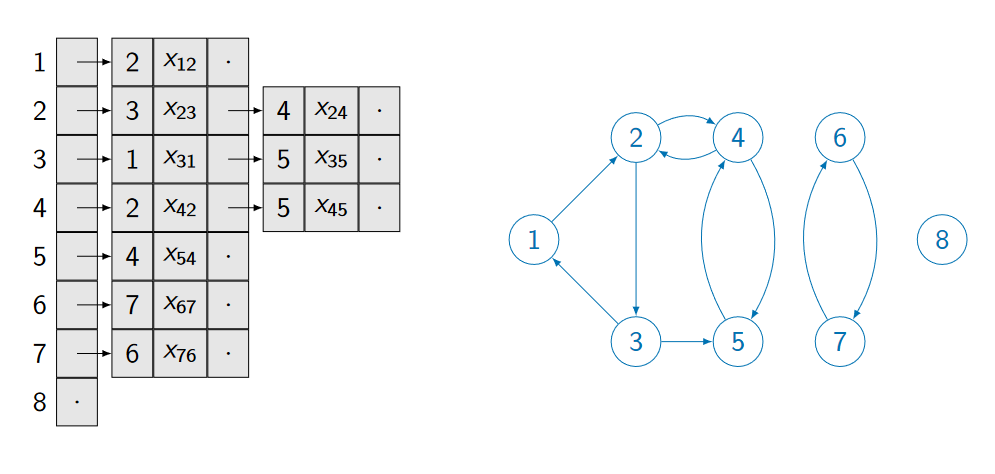
\includegraphics[width=.7\textwidth]{IMAGES/opti/optinetwork.png}
\end{figure}

\subsection{Transshipment}
Let's define $s_i = $div$(x)_i$.\\

This gives us the linear optimization problem : \\
$\min_{x\in \mathbb{R}^n} \sum_{(i,j)\in \mathcal{A}} c_{ij} x_{ij}$\\
subject to : $\sum_{j\lvert (i,j) \in \mathcal{A}} x_{ij} - \sum_{k\lvert (k,i) \in \mathcal{A}} x_{ki} = s_i$\\
$l_{ij} \leq x_{ij} \leq u_{ij}$\\

In order to solve this problem, we need to put it in standard form.\\
We define $x_{ij}' = x_{ij}-l_{ij} \geq 0$, $u_{ij}-l_{ij} = u_{ij}'$, and redefine the divergence of each vertices such that : $s_i = \sum_{j\lvert (i,j) \in \mathcal{A}} x_{ij}' -\sum_{k\lvert (k,i) \in \mathcal{A}} x_{ki}'$ (outgoing minus ingoing). Then, we compute the divergence for these sames nodes but now taking into account that we add a node in between each pair : \\
$s_{i}' = s_i - \sum_{(i,j)\in\mathcal{A}}u_{ij}$ \textbf{\warning Here we only subtract the outgoing maximum values of each outgoing arc as the minimum are set to zero.}\\

And set the lower bound $l_i'$ to zero.\\

The problem is now : \\

$\min_{x\in \mathbb{R}^n} \sum_{(i,j)\in \mathcal{A}} c_{ij}x_{ij}$\\
subject to : $\sum_{j\lvert (i,j) \in \mathcal{A}} x_{ij}' -\sum_{k\lvert (k,i) \in \mathcal{A}} x_{ki}' = s_i'$\\
$x_{ij}'\geq 0$\\

Or even : $\min_{x\in \mathbb{R}^n} c^Tx$\\
subject to $Ax=s$, $x\geq 0$\\
Here is a summary : 

\begin{figure}[hbt!]
    \centering
    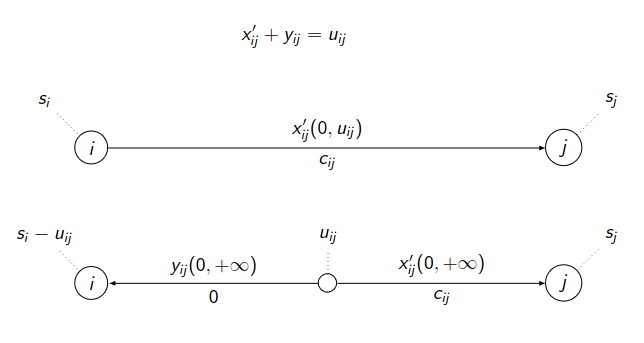
\includegraphics[width=.6\textwidth]{IMAGES/opti/Screenshot from 2024-01-13 21-55-37.png}
\end{figure}


Which for an example is : 
\\
\begin{figure}[hbt!]
    \centering
    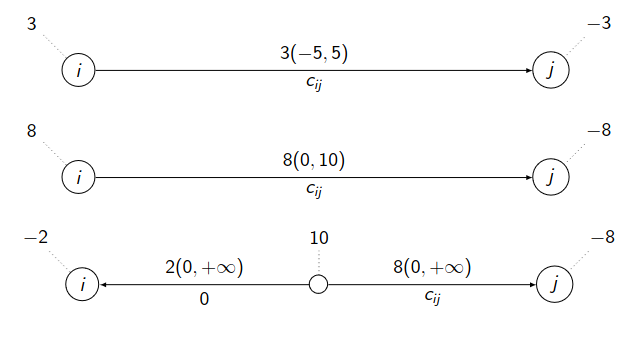
\includegraphics[width=.6\textwidth]{IMAGES/opti/Screenshot from 2024-01-13 21-57-11.png}
\end{figure}


\textbf{The matrix A (incidence matrix) is only composed of 1,-1,0}. For each arc $(i,j)$ of index k, $a_{ik}=1$ and $a_{jk} = -1$\\
The matrix A has nodes' number on each row and arcs' number on each column.\\

\warning \textbf{The final solutions are the variables corresponding to a non-zero cost; we do not take into account anymore the points in between and remove the variables corresponding to $c_{ij}=0$.}\\

The Lagrangian of the problem is given by : \begin{equation}
    L(x,\lambda,\mu) = \sum_{(i,j)\in \mathcal{A}} c_{ij}x_{ij} + \sum_{i\in \mathcal{N}} \lambda_i(\sum_{j\lvert (i,j) \in \mathcal{A}} x_{ij} - \sum_{k\lvert (k,i) \in \mathcal{A}} x_{ki} - s_i) - \sum_{(i,j)\in \mathcal{A}} \mu_{ij} x_{ij}
\end{equation}

In order to have a bounded problem, we need the coefficients of $x_{ij} = 0$ : $c_{ij} + \lambda_i - \lambda_j - \mu_{ij} = 0$ and $\mu_{ij} = 0$\\

\quad \underline{Total unimodularity :}\\
The incidence matrix defining the constraints of a transshipment problem has a special structure. It guarantees to generate an integer solution if the data is integer.\\

The optimal solution is as usual given by : $x_B^* = B^{-1}s$\\

\textbf{Cramer's rule :} \begin{equation}
    x_B^* = \frac{1}{det(B)}C B^Ts
\end{equation}
Each entry of the matrix is $0,1$ or $-1$. Each entry of $CB$ is an integer. If $s$ is an integer, $CB^Ts$ is an integer. Then if det$(B)$ is 1 or -1, $x_B^*$ is an integer.\\

\begin{theoremen}
    The matrix $A \in \mathbb{Z}^{mxn}$ is totally unimmodular if the determinant of each square sub-matrix of A is 0,1 or -1.\\
\end{theoremen}

Consider the polyhedron $\{x\in \mathbb{R}^n \lvert Ax=b, x\geq 0\}$. If A is totally unimodular, then every basic solution is integer.\\

\begin{theoremen}
    The incidence matrix of a transshipment network is totally unimodular.\\
\end{theoremen}

\begin{theoremen}
    If the supply vector $s$ of the transshipment problem is an integer and if the problem is bounded, then it has an optimal solution which is an integer.\\
\end{theoremen}

\warning A is usually not full rank as it will always have two (no more no less) 1 or -1 in each column. The rows are linearly dependant as one constraint is redundant (the sum of all divergence is equal to zero, therefore we can remove one constraint)\\

\subsubsection{Maximum flow problem}
We have a network where each arc has a capacity. What is the maximum amount of flow that the network can carry from o to d? We create an artificial arc between d and o : \begin{itemize}
    \item cost on the artificial arc : -1\\
    \item cost on every other arc : 0\\
    \item supply for each node 0\\
    \item lower bound on each arc : 0\\
    \item upper bound on the artificial one : $\infty$\\
\end{itemize}
The standard form : \\
$\min -x_{do}$\\
subject to : $\sum_{j\lvert (i,j)\in A} x_{ij} - \sum_{k\lvert (k,i) \in A} x_{ki} =0$\\
$0 \leq x_{ij} \leq u_{ij}$\\

\subsubsection{Transportation problem}
There is a cost to transport items from a supplier to a customer. There is no real network, we create a representation. One set of nodes for the suppliers and one set of nodes for the customers.\\
\begin{itemize}
    \item cost on each arc : $c_{ij}$\\
    \item supply for supplier nodes : $s_i$\\
    \item supply for customer nodes : $-t_j$\\
    \item lower bound on each arc : 0, upper : $\infty$\\
\end{itemize}

The standard form : \\
$\min \sum_{i=1}^{m_o} \sum_{j=1}^{m_d} c_{ij}x_{ij}$\\
subject to : \begin{itemize}
    \item $\sum_{j=1}^{m_d} x_{ij} = s_i$\\
    \item $\sum_{i=1}^{m_o} x_{ij} = t_j$\\
\end{itemize}

\subsubsection{The assignment problem}
It consists in assigning n tasks to n resources at minimal cost.
\begin{itemize}
    \item cost on each arc : $c_{ij} = -p_{ij}$\\
    \item supply for each resource node : 1\\
    \item supply for each task node : -1\\
    \item lower bound 0, upper 1\\
\end{itemize}

Standard form : \\
$\min \sum_{i=1}^n \sum_{j=1}^n c_{ij}x_{ij}$\\
subject to : \begin{itemize}
    \item $\sum_{j=1}^n x_{ij}=1$\\
    \item $\sum_{i=1}^n x_{ij}=1$\\
\end{itemize}


\subsection{Shortest path}
We consider here a forward path. Therefore, the cost associated is : $C(P) = \sum_{(i,j)\in P} c_{ij}x_{ij}$.\\

We also set the lower bound of each arc to 0 : $l_{ij} = 0$.\\

We send \textbf{one unit of flow from o to d}.\begin{itemize}
    \item cost of each arc : $c_{ij}$\\
    \item supply at origin : $s_0=1$\\
    \item supply at destination : $s_d=-1$\\
    \item supply at any other node : $s_i=0$\\
    \item lower bound on each arc $ 0$\\
    \item upper bound on each arc $\infty$/1(for simple path)\\
\end{itemize}
Therefore, the cost of a path is here : $C(P) = \sum_{(i,j)\in P} c_{ij}$\\

The standard form : \\
$\min \sum c_{ij}x_{ij}$\\
subject to : \begin{itemize}
    \item $\sum_{j\lvert (o,j)\in A} x_{oj} - \sum_{k\lvert (k,o) \in A} x_{ko} = 1$\\
    \item $\sum_{j\lvert (d,j)\in A} x_{dj} - \sum_{k\lvert (k,d) \in A} x_{kd} = -1$\\
    \item $\sum_{j\lvert (i,j)\in A} x_{ij} - \sum_{k\lvert (k,i) \in A} x_{ki} = 0$\\
\end{itemize}

\begin{theoremen}
    Consider a network (N,A), n arcs, m nodes. A cost vector $c\in \mathbb{R}^n$, a vector of labels $\lambda \in \mathbb{R}^m$. A path P between node o and node d : \begin{equation}
        \begin{gathered}
            \lambda_j \leq \lambda_i +c_{ij}, \quad \forall (i,j)\in A\\
            \lambda_j = \lambda_i + c_{ij}, \quad \forall (i,j)\in P\\
        \end{gathered}
    \end{equation}
    Then P is the shortest path from o to d.\\
\end{theoremen}

\warning In order to get the right expression, when doing the Lagrangian, always put the constant on the left side of the equation and not the other way around.\\

Usually, we normalize $\lambda_o = 0$\\

If there exists a forward path from o to d containing a negative cost cycle, no forward path is the shortest path from o to d (problem is unbounded as increasing the number of cycle would bring down the cost).\\

\begin{theoremen}
    If $c\geq 0$, then $C(P) \geq 0$. Otherwise, \begin{equation}
        C(P) \geq (m-1) \min c_{ij}
    \end{equation}
\end{theoremen}

For any $l=1,\dots, k$, the sub-path $P_{ol} = o \rightarrow \dots \rightarrow i_l$ is the shortest path from o to $i_l$ if P is the shortest path from o to d.\\

The label of node $j$ can be interpreted as the length of the shortest path identified from the origin to node j ($\lambda_j$).\\

\underline{Algorithm :} \\
$S\leftarrow \{o\}$, $\lambda_o = 0$, $\lambda_j = \infty$\\
\begin{itemize}
    \item Select i in S\\
    \item For each (i,j) : \begin{itemize}
        \item If $\lambda_j > \lambda_i + c_{ij}$ \begin{itemize}
            \item $\lambda_j = \lambda_i+  c_{ij}$\\
            \item If $\lambda_j < 0$ and $\lambda_j < (m-1)\min c_{ij}$ : STOP (negative cycle)\\
            \item $S \leftarrow S\cup \{j\}$\\
        \end{itemize}
    \end{itemize}
    \item $S\leftarrow S\backslash \{i\}$\\
    \item If $S = \emptyset$ : STOP\\
\end{itemize}

We have multiple results : \begin{itemize}
    \item If $i \in S$, then $\lambda_i \neq \infty$\\
    \item for each node i, the value of $\lambda_i$ does not increase during the iteration\\
    \item if $\lambda_i \neq \infty$, it is the length of one path from o to i\\
    \item if $i \notin S$ then, either $\lambda_i = \infty$ or $\lambda_j \leq \lambda_i + c_{ij}$\\
    \item if algorithm terminates with $S=\emptyset$ then we have $\lambda_j = \infty$ if and only if there is no path from o to j\\
\end{itemize}

\warning As $\lambda_j \leq c_{ij}+\lambda_i$, if we have the relation $\lambda_j< c_{ij}+\lambda_i$ then, the corresponding variable of the arc $x_{ij}$ has to be 0. Then, thanks to flow conservation, we can compute the rest of the variables.\\

\quad \underline{Bellman's equation :} by the end of the algorithm, we have \begin{equation}
    \lambda_j = \min(\lambda_i + c_{ij})
\end{equation}

\quad \underline{Bellman's sub-network :}\\
For each $j\neq o$, select one (i,j) verifying the equation. Because we have m nodes, there will be m-1 arcs. By definition there cannot be any cycle and therefore, there is only path from o to any i. The sub-network is called the shortest path tree.\\

\quad \underline{Dijkstra's algorithm :}\\
Cost on the arcs are all non negative. We only want to treat each node only once. There is also no cycle with negative cost and no need to check if the problem is unbounded.\\

\underline{Algorithm :}\\
\begin{itemize}
    \item $\lambda_o = 0$\\
    \item $\lambda_i = \infty$\\
    \item $S\leftarrow \{o\}$\\
    \item $\forall (i,j)$, if $\lambda_j > \lambda_i + c_{ij}$ : \begin{itemize}
        \item $\lambda_j = \lambda_i + c_{ij}$\\
        \item $S \leftarrow S\cup \{j\}$\\
    \end{itemize}
    \item $S \leftarrow S\backslash \{i\}$\\
\end{itemize}

\quad \underline{Permanent label :}\\
Nodes in T will never be in S again (test a node only once).\\

\begin{equation}
    \mathcal{T} = \{i \lvert \lambda_i \neq \infty \text{ and } i\notin \mathcal{S}\}
\end{equation}

\begin{itemize}
    \item If $i \in \mathcal{T}$ and $j\notin \mathcal{T}$, then $\lambda_i\leq \lambda_j$\\
    \item If $i \in \mathcal{T}$ at the beginning of the iteration, then the label $\lambda_i$ is not modified during the iteration\\
    \item If $i\in \mathcal{T}$ at the beginning of the iteration, then $i \notin \mathcal{S}$ at the end of the iteration\\
    \item If $i\in \mathcal{T}$, then $\lambda_i$ is the length of the shortest path from o to i\\
\end{itemize}

\subsubsection{Longest path}
Find a simple forward path between o and d with the maximal cost.\\

\begin{equation}
    \max \sum_{(i,j)\in \mathcal{A}} c_{ij}x_{ij} = \min \sum_{(i,j)\in \mathcal{A}} (-c_{ij})x_{ij}
\end{equation}

\subsubsection{PERT}
Program Evaluation and Review Technique\\

\begin{itemize}
    \item Project composed of m tasks\\
    \item Each task has a duration and has a list of predecessors (there is an order to respect)\\
    \item What is the minimum duration of the project : longest path\\
    \item What are the tasks that do not tolerate any delay without delaying the project : the ones on the longest path\\
\end{itemize}

\subsection{Discrete optimization}

Binary variable are convenient to model many situations.\\

Logical : \begin{itemize}
    \item Identity : $x = \begin{cases}
        1 & \text{ if P is true}\\
        0 & \text{ if P is false}\\
    \end{cases}$\\
    \item Negation : $\neg P : 1-x$\\
    \item Conjunction : (AND) $P\wedge Q : xy$\\
    \item Dis-junction : (OR) $P\vee Q : x+y\geq 1$\\
    \item Exclusive dis-junction : $P \oplus Q : x+y=1$\\
    \item Implication : $P\Rightarrow Q : x\leq y$ (equivalent to $\neg P\vee Q$)\\
    \item Equivalence : $P\Leftrightarrow Q : x=y$\\
\end{itemize}

z is a binary variable. We can define have some optional constraints : \begin{itemize}
    \item $\geq$ : \begin{itemize}
        \item If $z=1$, $f(x)\geq a$ must be verified\\
        \item If $z=0$, $f(x)\geq a$ must not be verified\\
        \item we assume $f$ is bounded from below by L : \begin{equation}
            f(x) \geq L+(a-L)z
        \end{equation}
    \end{itemize}
    \item $\leq$ : \begin{itemize}
        \item If $z=1$, $f(x)\leq a$ must be verified\\
        \item If $z=0$, $f(x)\leq a$ must not be verified\\
        \item we assume $f$ is bounded from above by M : \begin{equation}
            f(x) \leq az + (1-z)M
        \end{equation}
    \end{itemize}
\end{itemize}

We can also have some disjunctive constraints : $f(x)\geq a$ and $g(x) \geq b$, one of them must be verified, not both.\\
Also, $f$ and $g$ are bounded from below : $f(x)\geq L_f$ and $g(x)\geq L_g$.\\

Then : \begin{equation}
    \begin{gathered}
        f(x)\geq L_f + (a-L_f)z\\
        g(x) \geq Lg + (b-L_g)(1-z)\\
    \end{gathered}
\end{equation}

\subsubsection{Linearization}
We can linearize some non linear specification. For example, the logical conjunction (AND) $z=xy$ is equivalent to : $x+y\leq 1+ z$ and $z\leq x$ and $z\leq y$.\\

The binary linear optimization problem is : \\
$\min c^Tx$\\
subject to $Ax=b$, $x\in \{0,1\}^n$\\

In order to get a binary problem, we need to \textbf{transform the data : }\\

Consider $x\in \mathbb{N}$, $x\leq u$ \begin{equation}
    \begin{gathered}
        x = \sum_{i=0}^{K-1}2^iz_i\\
        K = \lceil \log_2(u+1)\rceil\\
    \end{gathered}
\end{equation}

Where $u$ is the number of elements.\\

\subsubsection{Combinatorial optimization}
We have : $\min f(x)$\\
subject to $x\in \mathcal{F}$ a large finite set.\\

Some classical combinatorial optimizations problem : \begin{itemize}
    \item Knapsack problem : backpack with capacity $W$kg, needs to choose between n items of utility $u_i$ and weight $w_i$. Let the decision variable be $x_i = \begin{cases}
        1 & \text{item i goes into the knapsack}\\
        0 & \text{otherwise}\\
    \end{cases}$ We therefore have : $\max f(x) = \sum_{i=1}^n u_ix_i$ subject to $\sum_{i=1}^nw_ix_i \leq W$\\
    \item Set covering problem : we want to complete a collection of sticker but can only buy packs. We define a set U of m elements containing the collection, each set that we buy is $S_i \subseteq U$ and $a_{ij} = 1$ if element j belongs to subset $S_i$. The decision variable is $x_i = \begin{cases}
        1 & \text{if subset i is selected}\\
        0 & \text{otherwise}\\
    \end{cases}$
    Therefore, we have : $\min f(x) = \sum_{i=1}^n c_ix_i$ subject to $\sum_{i=1}^n a_{ij}x_i \geq 1$\\
    \item The travelling salesman problem : n nodes representing cities, for any pair $(i,j)$ of cities the distance $c_{ij}$ is known. The decision variable is : $x_{ij} = \begin{cases}
        1 & \text{if j is visited just after i}\\
        0 & \text{otherwise}\\
    \end{cases}$
    We also need to implement a variable $y_i$ : the position of city i in the tour. Then for each i and j different from home : $x_{ij} \Rightarrow y_j \geq y_i+1$ or in other words : $x_{ij}(n-1) + y_i-y_j \leq n-2$ $\forall (i,j) \notin$ start city. The problem now becomes : \\
    $\min_{x\in \mathbb{Z}^{n(n-1)}, y \in \mathbb{Z}^{n-1}} \sum_{i=1}^n \sum_{j\neq i} c_{ij}x_{ij}$ subject to $\begin{matrix}
        \sum_{j\neq i} x_{ij} = 1\\
        \sum_{i \neq j} x_{ij} = 1\\
        x_{ij}(n-1) + y_i - y_j \leq n-2\\
    \end{matrix}$\\
\end{itemize}

\subsubsection{The curse of dimensionality}
\warning There is no optimality condition for discrete optimization. i.e. the solution might not be on a vertex.\\

Another problem is the number of possibilities that the algorithm has to try; for example the knapsack problem has $2^n$ possibilities.\\

\subsubsection{Relaxation}
There is a way to convert discrete optimization problem into linear ones: \textbf{relaxation}. If we forget the integrality constraints, we obtain a linear optimization problem that can be solved more easily.\\
For example : \\
\begin{minipage}{.49\textwidth}
    Original problem : \\
    $\min_{x \in \mathbb{R}^n, y \in \mathbb{Z}^n, z \in \mathbb{N}^n} f(x,y,z)$\\
    subject to \begin{itemize}
        \item $g(x,y,z) \leq 0$\\
        \item $g(x,y,z) = 0$\\
        \item $y\in \mathbb{Z}^n$\\
        \item $z\in \{0,1\}^n$\\
    \end{itemize}
\end{minipage}
\hfill
\begin{minipage}{.49\textwidth}
    Relaxation problem : \\
    $\min_{x \in \mathbb{R}^n, y \in \mathbb{Z}^n, z \in \mathbb{N}^n} f(x,y,z)$\\
    subject to \begin{itemize}
        \item $g(x,y,z) \leq 0$\\
        \item $g(x,y,z) = 0$\\
        \item $y\in \mathbb{R}^n$\\
        \item $z\in [0,1]^n$\\
    \end{itemize}
\end{minipage}

If the discrete optimization P has an optimal solution $(x^*, y^*, z^*)$ and the relaxation has an optimal solution $(x_R^*, y_R^*, z_R^*)$ then : \begin{equation}
    f(x_R^*, y_R^*, z_R^*) \leq f(x^*, y^*, z^*)
\end{equation}

Therefore, for mixed integer linear problems, calculate $(x^*_R, y^*_R, z^*_R)$ using the simplex algorithm and round the solution to the nearest integer values.\\
\warning This method might lead to only non-feasible solution even tough the problem has an optimal solution.\\

\subsubsection{Branch and Bound}
In the absence of optimality conditions, enumeration is the only way to find the optimal solution. But it is most of the time impossible to perform due to the curse of dimensionality.\\
We therefore introduce the branch and bound method.\\

We take the set $\mathcal{F}$ on which $x$ belongs and divide it into subsets. We then solve each problem separately : \\
$\min f(x)$ subject to $x\in \mathcal{F}_k$\\

\begin{theoremen}
    Consider $i$ such that $f(x_i^*)\leq f(x_k^*)$, k=$1,\dots, K$\\
    Then : $f(x^*) = f(x_i^*)$ and $x_i^*$ is solution of P\\
\end{theoremen}

\begin{theoremen}
    Consider i such that $f(x_i^*)\leq f(x_k^*)$, k=$1,\dots, M$\\
    and $f(x_i^*) \leq l(P_k)$, k=$M+1, \dots, K$\\
    Then $f(x^*) = f(x_i^*)$ and $x_i^*$ is solution of P.\\
\end{theoremen}

\quad \underline{Algorithm :}\\
\begin{itemize}
    \item Initialization : \begin{itemize}
        \item $U=+\infty$ or an upper bound U that is the value of the objective function at the best feasible solution encountered so far\\
        \item $S = \{P\}$\\
    \end{itemize}
    \item Iteration : \begin{itemize}
        \item Consider an active sub-problem $P_k$\\
        \item If $P_k$ is infeasible, remove it from the list, otherwise calculate a lower bound $l(P_k)$\\
        \item If $U\leq l(P_k)$ remove $P_k$ from the list. Otherwise : \begin{itemize}
            \item solve $P_k$ directly or partition its feasible set and create new sub-problems that are added to the list.\\
        \end{itemize}
    \end{itemize}
\end{itemize}

\subsection{Nonlinear optimization}
We want : $\min_{x\in \mathbb{R}^n} f(x)$ where $f$ is twice differentiable.\\
Sufficient and optimality conditions :\\
\begin{theoremen}
    Consider $x^*$ and $f : \mathbb{R}^n \rightarrow \mathbb{R}$ twice differentiable.\\
    If : \begin{equation}
    \begin{gathered}
        \nabla f(x^*) = 0\\
        \text{and } \nabla^2 f(x^*) > 0 \text{ or equivalently } \lambda_i > 0, i=1,\dots, n\\
        \end{gathered}
    \end{equation}
    Then $x^*$ is a local minimum of $f$.\\
\end{theoremen}

\begin{theoremen}
    $f : \mathbb{R}^n \rightarrow \mathbb{R}$ continuous, $x^* \in \mathbb{R}^n$ a local minimum of $f$.\\
    If $f$ is convex, then $x^*$ is a global minimum of $f$. If $f$ is strictly convex, then $x^*$ is the unique global minimum of $f$.\\
\end{theoremen}

\subsubsection{One variable, Newton's method}

\quad \underline{Taylor's theorem :}\\
$F : \mathbb{R} \rightarrow \mathbb{R}$ differentiable\\
\begin{equation}
    m_{\hat{x}}(x) = F(\hat{x}) + (x-\hat{x})F'(\hat{x})
\end{equation}

\quad \underline{Algorithm :}\\
At each iteration, find $x_{k+1}$ such that : $m_{\hat{x}} = 0 \Rightarrow x_{k+1} = x_k - \frac{F(x_k)}{F'(x_k)}$\\

\warning It doesn't always converge. But it is fast!\\

\quad \underline{Conditions to be met for convergence :}\\
\begin{itemize}
    \item $F'$ is Lipschits continuous : $\exists M>0$ such that $\forall x,y$, $\lvert F'(x) - F'(y) \rvert \leq M\lvert x-y\rvert$\\
    \item $\exists \rho >0$ such that $\lvert F'(x)\rvert \geq \rho$, $\forall x$\\
    \item $\exists \eta>0$ such that $\lvert x_0 - x^*\rvert < \eta$\\
\end{itemize}

\begin{theoremen}
    Consider the sequence of iterates : \begin{equation}
        x_{k+1} = x_k - \frac{F(x_k)}{F'(x_k)}
    \end{equation}
    $\lim_{k\rightarrow \infty} x_k = x^*$ and it converges q-quadratically : \begin{equation}
        \lvert x_{k+1} - x^*\rvert \leq \frac{M}{2\rho} \lvert x_k - x^*\rvert^2
    \end{equation}
\end{theoremen}

\subsubsection{N variables}

The linear model is : \begin{equation}
    m_{\hat{x}} (x) = F(\hat{x}) + J(\hat{x})(x-\hat{x})
\end{equation}

We can therefore do : \begin{equation}\begin{gathered}
    x_{k+1} = x_k + d_k\\
    J(x_k)d_k = -F(x_k)\\
    \end{gathered}
\end{equation}

We have the equivalence : \\
\begin{minipage}{.49\textwidth}
\underline{Equations :}\\
    Problem : \\
    \begin{equation}
        F(x) = 0
    \end{equation}
    Algorithm : $x_{k+1} = x_k + d_k$\\
    with $J(x_k) d_k = -F(x_k)$\\
\end{minipage}
\vline
\begin{minipage}{.5\textwidth}
\underline{Optimization :}\\
    Problem : \begin{equation}
        \nabla f(x) = 0
    \end{equation}
    Algorithm : $x_{k+1} = x_k + d_k$\\
    with $\nabla^2 f(x_k) d_k = -\nabla f(x_k)$\\
\end{minipage}

We can also define the \textbf{quadratic model} :\\
\begin{equation}
    m_{\hat{x}}(x) = f(\hat{x}) + (x-\hat{x})^T \nabla f(\hat{x}) + \frac{1}{2} (x-\hat{x})^T \nabla^2 f(\hat{x})(x-\hat{x})
\end{equation}
\warning $\nabla^2$ is the Hessian matrix !\\

\begin{itemize}
    \item \textbf{Newton's point} :$x_k \in \mathbb{R}^n$ such that $\nabla^2f(x_k)>0$, newton's point is defined as : $x_N = x_k + d_N$ with $\nabla^2 f(x_k) d_N = -\nabla f(x_k)$, descent direction if $\nabla f(x_k)^Td_N<0$\\
    \item \textbf{Cauchy's point} : $x_k$ such that $\nabla f(x_k)^T \nabla^2f(x_k) \nabla f(x_k) >0$, cauchy's point is defined as : $x_C = x_k - \alpha_C \nabla f(x_k)$ with $\alpha_C = \frac{\nabla f(x_k)^T \nabla f(x_k)}{\nabla f(x_k)^T \nabla^2 f(x_k) \nabla f(x_k)}$\\
\end{itemize}

\subsubsection{Descent methods}

\quad \underline{Preconditioning :}\\

We change the original problem with a change of variables in order to obtain a symmetric equation.\\

\begin{itemize}
    \item $H_k$ : symmetric positive definite\\
    \item $H_k = L_k L_k^T$ with $x' = L_k^Tx$ and $L_k$ a triangular inferior matrix.\\
    \item Steepest descent iteration is : $x_{k+1}' = x_k' - \alpha_k \nabla \Tilde{f}(x_k')$ : \begin{equation}
        x_{k+1} = x_k - \alpha_k H_k^{-1} \nabla f(x_k)
    \end{equation}
\end{itemize}

Finding a local optimum along a direction is difficult. We therefore need to choose a step that would decrease the function : $x_{k+1} = x_k + \alpha_k d_k$ where $\alpha_k$ is such that $f(x_{k+1})<f(x_k)$\\

Descent direction is a local concept. It assumes small steps. When steps are too long, Taylor's theorem dos not apply anymore. So we need to avoid long steps. We also want to avoid small steps as it produces almost no progress.\\

\begin{enumerate}
    \item \textbf{First Wolfe condition :} decrease proportional to the step (avoid long step) \begin{equation}
        f(x_k + \alpha_k d_k) \leq f(x_k) + \alpha_k \beta_1 \nabla f(x_k)^Td_k
    \end{equation}
    With $0<\beta_1<1$\\
    \item \textbf{Second Wolfe condition :} relative reduction of the derivative (avoid short step) \begin{equation}
        \nabla f(x_k+\alpha_k d_k)^Td_k \geq \beta_2 \nabla f(x_k)^Td_k
    \end{equation} With $0<\beta_2<1$\\
\end{enumerate}


\quad \underline{Compatibility of Wolfe conditions :}\\
\begin{theoremen}
    If $f$ is bounded from below along $d_k$, if $0<\beta_1<\beta_2<1$, then there exists $\alpha>0$ verifying both conditions.\\
\end{theoremen}

\quad \underline{Line search algorithm :}\\

If a step is too short, increase the step by an arbitrary factor $\lambda>1$. If it is too long, shorten it.\\
$\alpha$ has to be finite. Therefore, there is a finite number of iterations. \\

We can also combine Newton's method with the descents method as it will combine the pros of both methods.\\

Newton's method is a descent method where $\alpha_k = 1$ and $D_k = \nabla^2 f(x_k)^{-1}$ is positive definite.\\

If $\nabla^2 f(x_k)^{-1}$ is not positive definite, choose another $D_k$ : \begin{itemize}
    \item $D_k = I$ : not good as it has slow convergence\\
    \item $D_k(i,i)=\max(\varepsilon, \frac{\partial^2 f}{\partial x_i^2}(x_k))^{-1}$, with $\varepsilon>0$ and D diagonal\\
    \item Inflating $\nabla^2 f(x_k) : $ $D_k = (\nabla^2f(x_k) + \tau I)^{-1}$ where $\tau$ is calculated such that $D_k$ is positive definite.\\
\end{itemize}

If $\alpha_k = 1$ is not consistent with Wolfe conditions, apply the line search algorithm.\\









\end{document}